\chapter{Architecture}
\label{cha:arch}

This chapter describes how I organised the system after I had a working React laboratory and added a real evaluation path. I justified each split by what I needed to demonstrate, not by a catalogue of patterns.

\section{Overall architecture}
\label{sec:arch-overview}

Figure~\ref{fig:arch} shows the four processes I actually run.

\begin{figure}[htbp]
\centering
\begin{tikzpicture}[
  box/.style={draw, rounded corners, align=center, inner sep=6pt, font=\scriptsize, minimum width=3.1cm, minimum height=1.15cm},
  arr/.style={-{Stealth}, thick}
]
\node[box] (ui) at (0,0) {React UI\\Vite + four tabs};
\node[box] (ex) at (5.1,0) {Express\\ \texttt{server.ts}};
\node[box] (gem) at (5.1,2.3) {Gemini API\\ \texttt{gemini-3.5-flash}};
\node[box] (py) at (10.2,0) {Python eval\\FastAPI :8001};
\node[box] (m) at (10.2,-2.3) {CIFAR-10\\ResNet-56 weights};
\draw[arr] (ui) -- node[above, font=\scriptsize] {cookie / Basic + JSON} (ex);
\draw[arr] (ex) -- node[right, font=\scriptsize] {email / deepfake} (gem);
\draw[arr] (ex) -- node[above, font=\scriptsize] {\texttt{/attack}, \texttt{/health}} (py);
\draw[arr] (py) -- (m);
\end{tikzpicture}
\caption{Processes I used: the browser talks only to Express. Express talks to Gemini for teaching routes and to the Python service for real attacks.}
\label{fig:arch}
\end{figure}

I chose this split for a simple reason. The first application already had a React user interface and Express routes. Rewriting it as a notebook would have removed the laboratory that the examiners will click. Putting PyTorch inside Node would have been fragile. A second process on port 8001 lets me start or stop the attack service without taking the website down.

I run the Node application locally with \texttt{npm run dev} at \texttt{http://localhost:3000}. The real attack needs the Python service on port 8001.

\section{Client screens}
\label{sec:screens}

\texttt{App.tsx} keeps one \texttt{activeScreen} value: dashboard, phishing, deepfake, or adversarial. I chose a sidebar instead of separate deployments because the point of the project is one workflow.

The dashboard reads \texttt{phishingHistory}. It does not call the Python service. The phishing lab calls \texttt{/api/generate-phishing} and \texttt{/api/analyze-email}. The deepfake lab calls \texttt{/api/analyze-media-deepfake}. The attack lab calls \texttt{/api/adversarial-perturb}.

\section{Sequence: generate phishing}
\label{sec:seq-phish}

Figure~\ref{fig:seq-phish} is the generate path.

\begin{figure}[htbp]
\centering
\begin{tikzpicture}[
  every node/.style={font=\scriptsize},
  obj/.style={font=\scriptsize\bfseries},
  arr/.style={-{Stealth}}
]
\node[obj] (c) at (0,0) {Browser};
\node[obj] (s) at (4.0,0) {Express};
\node[obj] (g) at (8.0,0) {Gemini};
\draw (0,-0.3) -- (0,-5.4);
\draw (4.0,-0.3) -- (4.0,-5.4);
\draw (8.0,-0.3) -- (8.0,-5.4);
\draw[arr] (0,-0.8) -- node[above] {POST /api/generate-phishing} (4.0,-0.8);
\draw[arr] (4.0,-1.5) -- node[above] {injection / rate limit} (0,-1.5);
\node at (2.0,-1.9) {400 or 429 if rejected};
\draw[arr] (4.0,-2.5) -- node[above] {generateContent} (8.0,-2.5);
\draw[arr] (8.0,-3.3) -- node[above] {JSON email} (4.0,-3.3);
\draw[arr] (4.0,-4.1) -- node[above] {source=gemini} (0,-4.1);
\draw[arr] (4.0,-4.9) -- node[above] {on error: source=fallback} (0,-4.9);
\end{tikzpicture}
\caption{Generate-phishing sequence. A rejected prompt never reaches Gemini. A Gemini failure still returns a template.}
\label{fig:seq-phish}
\end{figure}

I kept the fallback because a viva demonstration should not die on a 503 from the model API. The source field is what stops that fallback from looking like a model measurement.

The analyse-email sequence is the same shape. The request body is \texttt{subject}, \texttt{body}, and optional \texttt{sender}. The success payload is \texttt{analysis} plus \texttt{source}.

\section{Sequence: deepfake scenario}
\label{sec:seq-df}

I implemented a branch before Gemini.

\begin{enumerate}
\item The browser posts \texttt{fileName}, \texttt{mediaType}, and \texttt{promptAnalysis}.
\item Express lowercases the filename. If it equals \texttt{ceo\_keynote\_urgent\_wire.mp4}, \texttt{financial\_analyst\_voicemail.wav}, or \texttt{id\_verification\_passport.png}, it returns the matching object from \texttt{PRE\_BAKED\_DEEPFAKES} with \texttt{source: "preset"}.
\item Otherwise it calls Gemini. On success the source is \texttt{gemini}. On error the source is \texttt{fallback} and \texttt{getDynamicFallbackDeepfake} builds a story from the filename and the word ``urgent''.
\end{enumerate}

No step reads an uploaded byte stream. I chose filename matching because it is deterministic for the three viva presets and because I did not have a licensed detector I could defend.

\section{Sequence: adversarial attack}
\label{sec:seq-adv}

Figure~\ref{fig:seq-adv} is the only path that I treat as computed.

\begin{figure}[htbp]
\centering
\begin{tikzpicture}[
  every node/.style={font=\scriptsize},
  obj/.style={font=\scriptsize\bfseries},
  arr/.style={-{Stealth}}
]
\node[obj] (c) at (0,0) {Browser};
\node[obj] (s) at (3.7,0) {Express};
\node[obj] (p) at (7.6,0) {FastAPI};
\node[obj] (m) at (11.0,0) {ResNet-56};
\draw (0,-0.3) -- (0,-5.0);
\draw (3.7,-0.3) -- (3.7,-5.0);
\draw (7.6,-0.3) -- (7.6,-5.0);
\draw (11.0,-0.3) -- (11.0,-5.0);
\draw[arr] (0,-0.9) -- node[above] {POST /api/adversarial-perturb} (3.7,-0.9);
\draw[arr] (3.7,-1.8) -- node[above] {POST /attack + token} (7.6,-1.8);
\draw[arr] (7.6,-2.7) -- node[above] {forward + FGSM/PGD} (11.0,-2.7);
\draw[arr] (11.0,-3.5) -- node[above] {softmax} (7.6,-3.5);
\draw[arr] (7.6,-4.3) -- node[above] {source=computed or 503} (0,-4.3);
\end{tikzpicture}
\caption{Adversarial sequence. If FastAPI is down, Express returns 503. Gemini is not called.}
\label{fig:seq-adv}
\end{figure}

\texttt{getAdversarialFallback} still exists in \texttt{server.ts}. I did not wire it to the POST handler. I left it unused on purpose so that a missing eval service cannot look like a successful attack.

\section{Data model}
\label{sec:data-model}

There is no database. I stored laboratory state in React \texttt{useState} hooks. Figure~\ref{fig:data} lists the fields.

\begin{figure}[htbp]
\centering
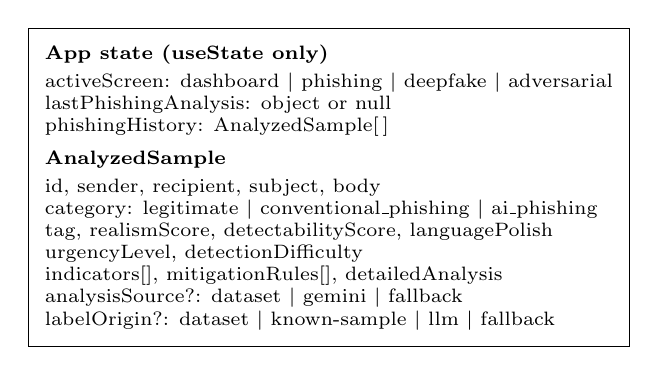
\begin{tikzpicture}[
  card/.style={draw, rectangle, align=left, font=\scriptsize, inner sep=6pt}
]
\node[card] (a) {
\textbf{App state (useState only)}\\[2pt]
activeScreen: dashboard $|$ phishing $|$ deepfake $|$ adversarial\\
lastPhishingAnalysis: object or null\\
phishingHistory: AnalyzedSample[\,]\\[4pt]
\textbf{AnalyzedSample}\\[2pt]
id, sender, recipient, subject, body\\
category: legitimate $|$ conventional\_phishing $|$ ai\_phishing\\
tag, realismScore, detectabilityScore, languagePolish\\
urgencyLevel, detectionDifficulty\\
indicators[], mitigationRules[], detailedAnalysis\\
analysisSource?: dataset $|$ gemini $|$ fallback\\
labelOrigin?: dataset $|$ known-sample $|$ llm $|$ fallback
};
\end{tikzpicture}
\caption{Client data model. Clearing the dataset only empties the React array.}
\label{fig:data}
\end{figure}

I chose client state because the 90 rows are generated in the browser from a seed. A database would have implied persistence that I do not have. The footer says the session is in memory. There is no PostgreSQL or SQLite.

The Python side keeps CIFAR-10 on disk under \texttt{eval/adversarial/results/cifar10/} after the first download. That cache is local data for the model, not a user database.

\section{API contracts}
\label{sec:api}

All JSON bodies are limited to 32\,kB. POST routes under \texttt{/api/} are rate limited. Table~\ref{tab:api} is the contract I implemented.

\begin{table}[htbp]
\centering
\caption{HTTP contracts for the four POST routes and the evaluation health route.}
\label{tab:api}
\scriptsize
\begin{tabular}{p{3.4cm}p{4.2cm}p{4.6cm}}
\toprule
Route & Request body & Success / error \\
\midrule
\texttt{POST /api/generate-phishing} & \texttt{scenario}, \texttt{promptText}, \texttt{customPrompt}, \texttt{complexity} & \texttt{\{success, source, email\}} with subject, body, realismScore, spoofingIndicators, mitigationRules. 400 if injected. 429 if limited. \\
\texttt{POST /api/analyze-email} & \texttt{subject}, \texttt{body}, \texttt{sender} & \texttt{\{success, source, analysis\}} with scores, predictedCategory, categoryRationale, indicators, mitigationRules, detailedAnalysis. \\
\texttt{POST /api/analyze-media-deepfake} & \texttt{fileName}, \texttt{mediaType}, \texttt{promptAnalysis} & \texttt{\{success, source, deepfakeAnalysis\}} with facialIrregularities, audioAnomalies, simulatedClassification, markers, actionableDefences. \\
\texttt{POST /api/adversarial-perturb} & \texttt{originalClass}, \texttt{targetClass}, \texttt{noiseLevel}, \texttt{architecture} & \texttt{\{success, source: computed, perturbation\}} or 502/503. No Gemini fallback. \\
\texttt{GET /api/eval/health} & none & Forwards Python \texttt{/health}. 503 if the service is down. \\
\bottomrule
\end{tabular}
\end{table}

I also added two GET helpers that only send a file if it exists: \texttt{/api/eval/phishing} and \texttt{/api/eval/adversarial}. They are not extra attack surfaces in the teaching sense. They just expose the JSON I need for Chapter~\ref{cha:eval}.

The Python \texttt{POST /attack} body is the same class pair plus \texttt{method} (default \texttt{fgsm}). If \texttt{EVAL\_INTERNAL\_TOKEN} is set, Express sends it as \texttt{X-Eval-Token}.

\section{Security controls in the request path}
\label{sec:arch-sec}

I placed three Express middleware checks in front of the routes: JSON size, \texttt{requireLabAccess}, and \texttt{rateLimitApi}. The generate-phishing handler then calls \texttt{promptLooksInjected} on the custom prompt and the prompt text. Chapter~\ref{cha:disc} maps those controls to STRIDE.
